\documentclass[a4paper, 12pt, french]{article}
\usepackage[utf8]{inputenc}
\usepackage[T1]{fontenc}
\usepackage{babel}

%Images
\usepackage{graphicx} 
\graphicspath{{src/dev/}}

%Code
\usepackage{listings}
\usepackage{color}

\definecolor{dkgreen}{rgb}{0,0.6,0}
\definecolor{gray}{rgb}{0.5,0.5,0.5}
\definecolor{mauve}{rgb}{0.58,0,0.82}

\lstset{frame=tb,
  language=C,
  aboveskip=5mm,
  belowskip=5mm,
  framesep=3mm,
  showstringspaces=false,
  columns=flexible,
  basicstyle={\small\ttfamily},
  numbers=none,
  numberstyle=\tiny\color{gray},
  keywordstyle=\color{blue},
  commentstyle=\color{dkgreen},
  stringstyle=\color{mauve},
  breaklines=true,
  breakatwhitespace=true,
  tabsize=3
}

%Commandes perso
\newcommand{\hr}{\noindent\rule{13.7cm}{0.4pt}}

%Metas
\title{Reseau}
\author{Elanis - https://github.com/Elanis/LaTeX-cheatsheets}
\date{}

\begin{document}
	\maketitle

	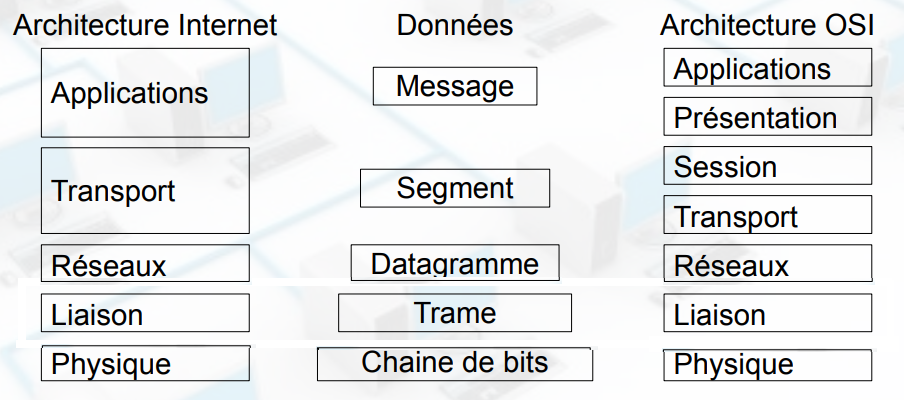
\includegraphics[width=13.8cm]{reseau_modele_osi}

	\section{Introduction}

	« Un réseau est un ensemble d'équipement reliés entre eux et qui échangent des informations »

	\subsection{Echanges sur de longues distances}
	\begin{itemize}
		\item Satellite
		\item Hertzien (TV)
		\item Cable aerien
		\item Antenne Parabolique
		\item Paire torsadée (ADSL, Telephone, etc)
		\item WiMax, Telephonique (2G, 3G, 4G), etc
		\item ...
	\end{itemize}

	\subsection{Echanges sur de courtes/moyennes distances}
	\begin{itemize}
		\item CPL (Courant porteur de ligne): Passage du signal par le reseau éléctrique
		\item NFC (Sans contact): Telephones, Cartes bancaires, Badges, etc
		\item Radio: Bluetooth, WiFi, etc
		\item Femtocell: mini-relai telephonique
		\item Ethernet (de 10 Mbps à 10 Gbps)
		\item ...
	\end{itemize}
	
	\subsection{Internet Mobile}  
	\begin{description}
		\item[2G] GSM/GPRS/EDGE - 384Kbps $\downarrow$ - 188.4Kbps $\uparrow$ - 900-1800 Mhz
		\item[3G] UMTS/3G+ (HSPA+) - 14.4Mbps $\downarrow$ - 5.7Mbps $\uparrow$ - 1900-2100 Mhz
		\item[4G] 4G (LTE) - 100Mbps $\downarrow$ - 50Mbps $\uparrow$ - 800 - 1800 - 2600 Mhz
	\end{description}

	\subsection{Internet Fixe}  
	\begin{description}
		\item[ADSL] 13.7Mbps $\downarrow$
		\item[ADSL 2] 25Mbps $\downarrow$
		\item[VDSL 2] 120Mbps $\downarrow$
		\item[Fibre optique] 200Mbps $\downarrow$
		\item[Internet par satellite] 20Mbps $\downarrow$ - \emph{Note:} Utilisée principalement dans les zones non reliables par les solutions précédentes.
	\end{description}

	\subsection{Le Cloud}

	Le but du cloud esst de "dématerialiser" les systèmes informatiques en les envoyant sur le Web. Il en résulte des problèmes sur le reseau avec tout ce nouveau traffic qui auparavant était local aux reseaux d'entreprise le plus souvent. Il exite néanmoins des solutions:

	\subsubsection{Le Edge Computing}

	L'edge computing est une méthode d'optimisation employée dans le cloud computing qui consiste à traiter les données à la périphérie du réseau, près de la source des données. Il est ainsi possible de minimiser les besoins en bande passante entre les capteurs et les centres de traitement des données en entreprenant les analyses au plus près des sources de données.

	\subsubsection{Le Fog Computing}

	Le fog computing consiste à exploiter des applications et des infrastructures de traitement et de stockage de proximité, servant d'intermédiaire entre des objets connectés et une architecture cloud classique.

	\subsection{Niveaux de service}

	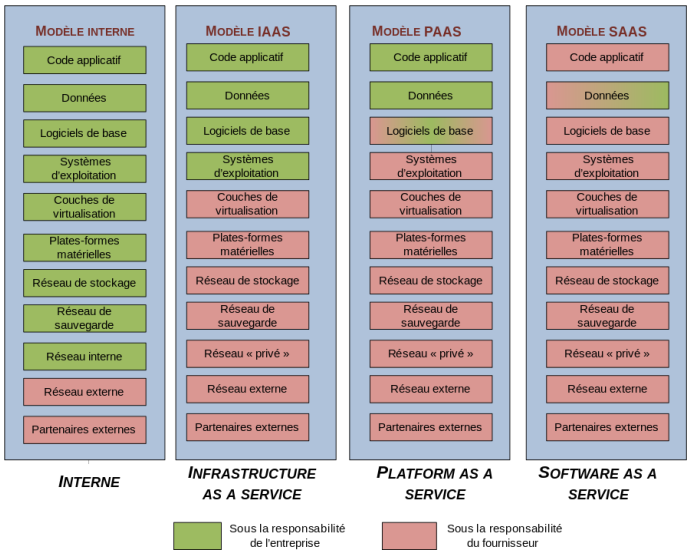
\includegraphics[width=13.8cm]{reseau_niveaux_de_service}

	\section{Physique}

	\emph{Bande passante:} Taille de la bande de frequence utilisée pour transmettre des données

	\emph{Attenuation: } Diminution du signal sur la distance

	\subsection{Supports de transmissions}

	\emph{Particularités diverses: } Bande passante, attenuation, sensibilité, coût, facillité d'installation, etc

	\begin{description}
		\item[Paire torsadée:] dans un même câble par 2, 4 ou 8 fils; une paire est un lien de communication. Chaque paire est enroulée pour limiter les interferences. \emph{Debit Max: 100 Gbps}. Simple, economique, reutilisable, mais sensible aux pertubations électromagnetiques et grande atténuation.
		\item[Coaxial:] il consiste en deux conducteurs ayant le même axe. \emph{Debit Max: 2 Gbps} Tres bonne qualité, haut debit, bonne manipulation mais très cher.
		\item[Fibre optique:] Cylindre de fibre de sillicium extremement fin. \emph{Debit Max: plusieurs terabits par seconde} Bande passante immense, debits très importants, insensibles aux interferences et corrosions chimiques, attenuation faible, leger mais fragile, unidirectionnel, transmission point à point, cout élevé des interfaces.
		\item[Ondes radio:] Wifi (56Mbps), Bluetooth (2Mbps), Infrarouge, Hertzien, etc \emph{Portée jusqu'a quelques centaines de mêtres}
		\item[Micro ondes:] Transmission terrestre de 50 à 1000km et satellitaire a 36000km (geostationnaire) ou 800 km d'altitude
	\end{description}


	\subsection{Transmission}

	\subsubsection{Caracteristiques d'un signal}

	Chacun se decompose en une somme infinie de sinusoides (decompostion de Fourrier)

	\emph{Note:} Tout ce qui est hors de la bande passante est naturellement filtré.  

	Rapport signal sur bruit(dB) $ = 10 * log_{10} \frac{S}{B}$ où S est la puissance du signal et B celle du bruit.

	\subsubsection{Capacité d'un canal de transmission}

	\emph{Theoreme de Shannon:} Soient W la bande passante d'un canal de transmission et S/B le rapport signal sur bruit. La capacité en bit/s du canal est :

		$$C = W * log_2 \left( 1 + \frac{S}{B} \right)$$

	\subsection{Numerisation, Quantification, Echantillonnage}

	\emph{Analogique:} Signal continu

	\emph{Numerique:} Signal echantilloné (sur le temps), et quantifié (sur les valeurs) afin d'être stockées et transmises par un equipement electronique.

	\subsubsection{Echantillonnage}

	\emph{Theoreme de Shannon:} Prendre comme max 2 fois la frequence max relevée

	\subsubsection{Quantification}

	Utilisation d'echelles logarithmiques

	\subsubsection{Formules}


	\begin{description}
		\item[Debit binaire ($D_b$)] Nombre max d'elements binaires transmis par seconde
			$$D_r = 1/T_b \ bit/s$$
		\item[Rapidité de modulation ($R_s$)] Vitesse à la queles les symboles se succèdent
			$$ R_s = 1/T_s  \ bauds$$
		\item[Valence (V)] Cardinal de l'alphabet des symboles
			$$ D = R_s * r = R_s * log_2 * V $$
		\item[Debit binaire max] Donne le debit binaire maximum en fonction de la bande passande du canal
			$$ D_{max} = 2 * W * log_2 * V $$
			où W est la largeur de la bande passante et V la valence du signal
	\end{description}

	\subsection{Transmission en bande de base}

	On transmet en bande de base, quand on transmet directement l'information codée sous forme d'un signal carré.

	\begin{description}
		\item[Tout ou rien] 0 est 0 Volt, 1 est +x Volts
		\item[Bipolaire] 0 est 0 Volts, 1 est alternativement +x ou -x Volts. \emph{Permet de mieux distinguer les suites de 1}
		\item[NRZ (No return to zero)] 0 est -x Volts, 1 est +x Volts. \emph{Permet de differencier le silence des 0}
		\item[NRZI (NRZ Inverted space)] 0 est un changement de niveau (entre +x et -x Volts), 1 correspond à une absence de changement.
		\item[RZ (Return to zero)] 0 est 0 Volts, 1 est un front montant (impulsion au milieu du temps bit)
		\item[Biphasé (ou Manchester)] 0 est un front montant, 1 est un front descendant. \emph{Il est plus facile a distinguer grace a un changement de signe à chaque bit}
		\item[Code manchester différentiel] 0 est un front inversé au cycle précédent, 1 est le même front que le cycle précédent.
		\item[Code Miller] 0 est une absence de changement sur l'intervalle, 1 est un front montant/descendant sur l'intervalle
 	\end{description}

	\subsection{Transmission modulée}

	Le principal problème de la transmission en bande de base est que le signal se degrade sur la distance, il est donc utilisé uniquement sur des reseaux locaux. On utilise donc pour de plus grandes distances des signaux sinuisoidaux générés et recupérés par des modems (modulateur - demodulateur).

	Afin d'y introduire de l'information, les modulations permettent de transformer:
	\begin{itemize}
		\item L'amplitude
		\item La fréquence
		\item La phase
	\end{itemize}

	\subsubsection{Modulation d'amplitude}

	Il s'agit d'associer un symbole à chaque amplitude.

	\emph{Avantages:} Moins couteux et plus précis qu'un signal carré, la modulation d'amplitude est simple.
	
	\emph{Désavantages:} Sensibles aux perturbations électromagnétiques (orage, ligne éléctrique, ...)

	\subsubsection{Modulation de fréquence}

	Il s'agit d'associer un symbole à chaque fréquence.

	\emph{Avantages:} Moins couteux et plus précis qu'un signal carré, résistant aux pertubations (d'amplitude).
	
	\emph{Désavantages:} Système de démodulation moins simple à concevoir

	\subsubsection{Modulation de phase}

	Il s'agit d'associer un symbole à des changements de phases.

	\emph{Avantages:} Les dispositifs de (dé)modulation de phase permettent de coder facilement deux états, résistant aux pertubations (d'amplitude).
	
	\emph{Désavantages:} Système de démodulation pas simple à concevoir

	\subsubsection{Combinaison de modulations}

	Les transmissions modulées peuvent combiner plusieurs formes de modulations simultanées. On représente ces modulations par un diagramme spatial:

	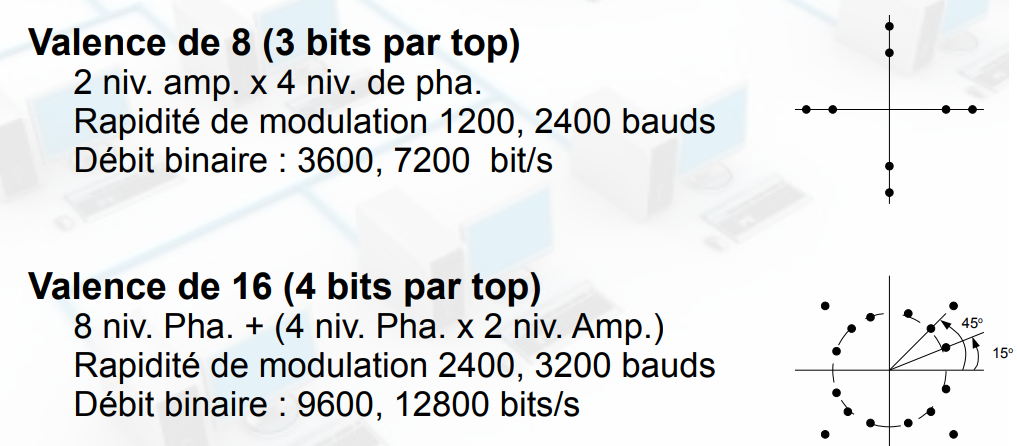
\includegraphics[width=13.8cm]{reseau_diagramme_spatial}
\end{document}